% ==================== CHƯƠNG 9 ====================
\newpage
\chap{Kết quả phân tích: trả lời các câu hỏi nghiệp vụ}\label{sec:results}
Mục này dùng kho dữ liệu và dashboard để trả lời các câu hỏi ở mục~\ref{sec:questions}. Tất cả số liệu được truy vấn từ kho \code{dw} (toàn bộ 2011--2012 nếu không ghi khác); các hình được sinh tự động bằng \code{report/scripts/make\_figures.py}.

\sect{Nhóm 1 - Phân tích nhu cầu sử dụng}

\noindent\textbf{Q1.1 - Tổng lượt thuê.} Hai năm có \textbf{3.292.679} lượt thuê (17.379 giờ, 731 ngày), trung bình 189,5 lượt/giờ. Năm 2011 có 1.243.103 lượt, năm 2012 có 2.049.576 lượt - \textbf{tăng 64,9\%}, cho thấy hệ thống đang tăng trưởng mạnh; điều này cũng là lý do DSS cho phép chọn kỳ lịch sử gần nhất.

\begin{table}[H]
\centering
\caption{Tám KPI trên toàn bộ dữ liệu}
\label{tab:kpi-values}
\begin{tabular}{|l|r|l|}
\hline
\textbf{KPI} & \textbf{Giá trị} & \textbf{Ghi chú} \\ \hline
Total Rentals & 3.292.679 & 2011: 1.243.103; 2012: 2.049.576 \\ \hline
Average Hourly Rentals & 189,5 & lượt/giờ \\ \hline
Peak Hour & 17h & TB 461,5 lượt/giờ \\ \hline
Lowest Demand Hour & 4h & TB 6,4 lượt/giờ \\ \hline
Registered User Ratio & 81,2\% & 2.672.662 lượt \\ \hline
Casual User Ratio & 18,8\% & 620.017 lượt \\ \hline
Working Day Demand & 4.585 & lượt/ngày (500 ngày) \\ \hline
Non-working Day Demand & 4.330 & lượt/ngày (231 ngày) \\ \hline
\end{tabular}
\end{table}

\noindent\textbf{Q1.2 - Khung giờ cao nhất và thấp nhất.} Trên toàn bộ dữ liệu, giờ cao điểm là \textbf{17h} (461,5 lượt/giờ) và giờ thấp nhất là \textbf{4h} (6,4 lượt/giờ) - chênh lệch hơn 70 lần. Hình~\ref{fig:hourly} cho thấy hồ sơ theo giờ khác hẳn giữa hai loại ngày: ngày làm việc có hai đỉnh nhọn lúc 8h (477) và 17h (525); ngày nghỉ có một đỉnh tròn lúc 12--14h (khoảng 370).

\begin{figure}[H]
\centering
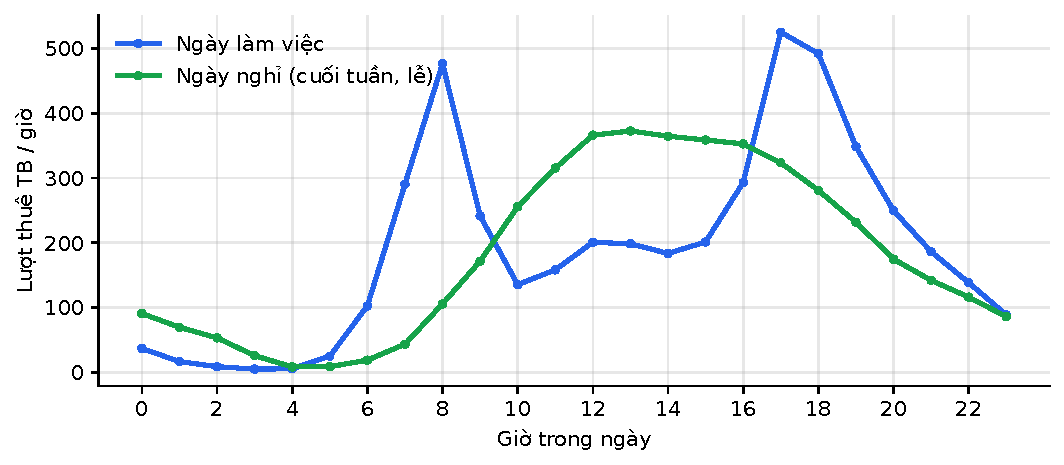
\includegraphics[width=0.95\textwidth]{figures/hourly_profile.pdf}
\caption{Lượt thuê trung bình theo giờ: ngày làm việc và ngày nghỉ}
\label{fig:hourly}
\end{figure}

\noindent\textbf{Q1.3 - Khác biệt giữa các ngày trong tuần.} Năm 2011 nhu cầu trung bình/giờ gần như đều giữa các thứ (137,6--147,6). Năm 2012 có khác biệt rõ hơn: thấp nhất Chủ nhật (210,0), cao nhất thứ Năm (249,5). Khác biệt lớn nhất nằm ở \textbf{thành phần người dùng} (Hình~\ref{fig:users}): người dùng vãng lai chiếm 31,6\% (Chủ nhật) và 32,2\% (thứ Bảy), nhưng chỉ 12--16\% vào các ngày trong tuần.

\begin{figure}[H]
\centering
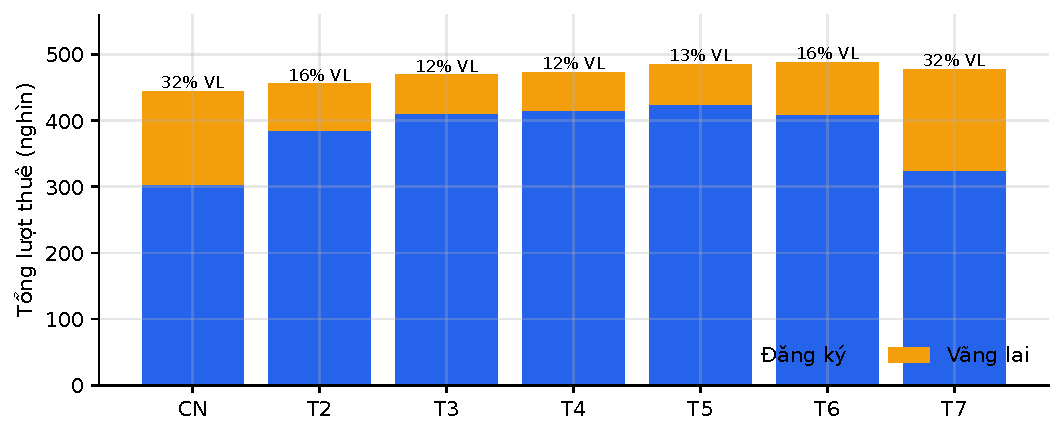
\includegraphics[width=0.92\textwidth]{figures/users_weekday.pdf}
\caption{Lượt thuê theo thứ trong tuần và tỷ lệ người dùng vãng lai (VL)}
\label{fig:users}
\end{figure}

\noindent\textbf{Q1.4 - Theo mùa và tháng.} Theo mùa (mã mùa của nguồn), mùa 3 (Fall) có tổng lượt thuê cao nhất (1.061.129), sau đó là Summer (918.589), Winter (841.613) và thấp nhất Spring (471.348) - lưu ý mùa ``Spring'' của nguồn ứng với khoảng 21/12 -- 20/3, tức thực tế là mùa đông lạnh nhất. Theo tháng (Hình~\ref{fig:monthly}), nhu cầu thấp nhất vào tháng 1, tăng dần đến đỉnh mùa hè - thu (2011: tháng 6, 199,3 lượt/giờ; 2012: tháng 9, 303,6 lượt/giờ) rồi giảm vào cuối năm. Đường 2012 nằm trên đường 2011 ở mọi tháng.

\begin{figure}[H]
\centering
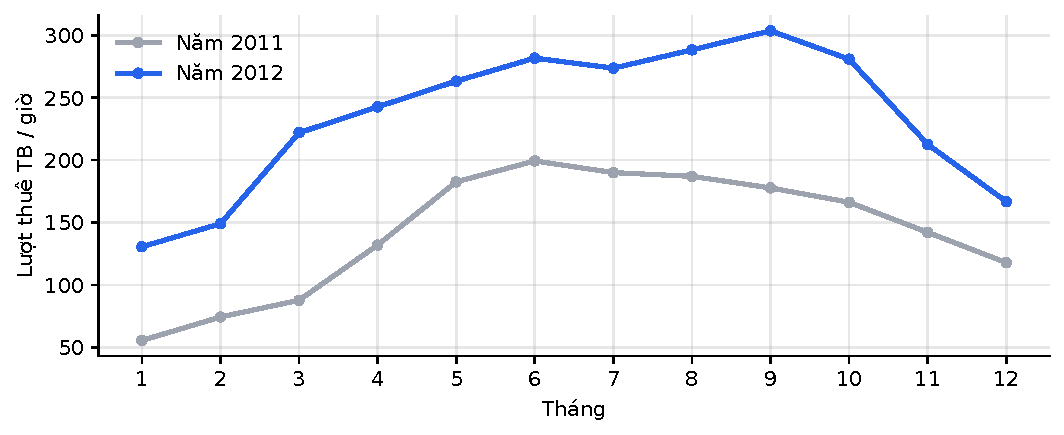
\includegraphics[width=0.92\textwidth]{figures/monthly_trend.pdf}
\caption{Lượt thuê trung bình/giờ theo tháng, so sánh hai năm}
\label{fig:monthly}
\end{figure}

\noindent\textbf{Q1.5 - Tỷ lệ người dùng.} Người dùng đăng ký chiếm \textbf{81,2\%} lượt thuê, vãng lai \textbf{18,8\%}. Tỷ lệ vãng lai thay đổi mạnh theo giờ: chỉ 5,5\% lúc 6h nhưng 29,8\% lúc 15h - người đăng ký chủ yếu dùng xe để đi làm, người vãng lai dùng xe để giải trí vào buổi chiều và cuối tuần.

\sect{Nhóm 2 - Ảnh hưởng của các yếu tố}

\noindent\textbf{Q2.1 - Thời tiết.} So với trời quang (204,9 lượt/giờ), trời sương mù làm nhu cầu giảm 14,5\% (175,2) và mưa/tuyết nhẹ làm giảm 45,5\% (111,6). Mức mưa lớn chỉ có 3 giờ quan sát (74,3) nên không đủ tin cậy để kết luận (Hình~\ref{fig:weather}, cột màu xám).

\begin{figure}[H]
\centering
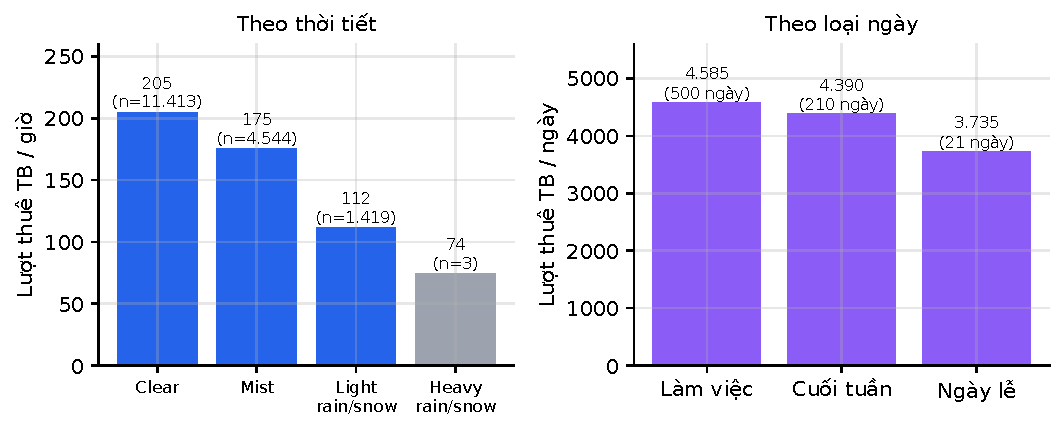
\includegraphics[width=0.95\textwidth]{figures/weather_daytype.pdf}
\caption{Lượt thuê trung bình theo thời tiết (theo giờ) và theo loại ngày (theo ngày)}
\label{fig:weather}
\end{figure}

\noindent\textbf{Q2.2 - Nhiệt độ và độ ẩm.} Nhiệt độ có tương quan \textbf{dương} với nhu cầu: $r = 0{,}41$ ở mức giờ và $r = 0{,}63$ ở mức ngày. Nhu cầu tăng đều từ 48,6 lượt/giờ (0--5$^\circ$C) lên 330,3 (30--35$^\circ$C), rồi giảm nhẹ khi trên 35$^\circ$C (318,5). Độ ẩm có tương quan \textbf{âm}: $r = -0{,}33$ ở mức giờ, nhu cầu giảm từ khoảng 300 lượt/giờ (độ ẩm 20--30\%) xuống 80,8 (90--100\%). Tuy nhiên ở mức ngày tương quan chỉ còn $r = -0{,}11$: phần lớn quan hệ theo giờ là do \textbf{biến gây nhiễu} giờ trong ngày (ban đêm vừa ẩm hơn vừa vắng khách). Phân tích độ ẩm dùng 17.357 giờ: 22 giờ độ ẩm 0\% (lỗi cảm biến, \code{humidity\_pct = NULL}) bị loại; khoảng 0--10\% chỉ còn 1 giờ nên được gắn cờ ít mẫu. Tương quan không đồng nghĩa nhân quả (Hình~\ref{fig:climate}).

\begin{figure}[H]
\centering
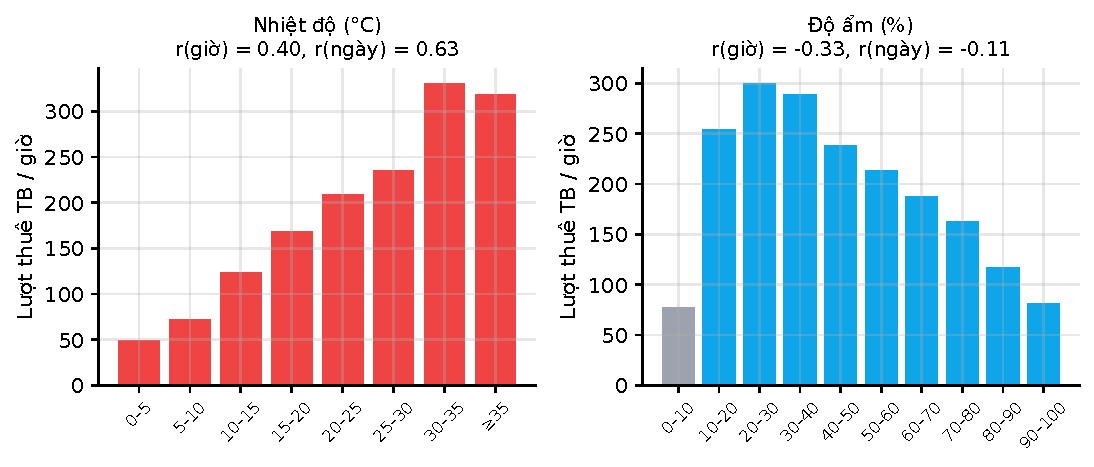
\includegraphics[width=0.95\textwidth]{figures/climate.pdf}
\caption{Lượt thuê trung bình/giờ theo khoảng nhiệt độ và độ ẩm (cột xám: dưới 30 giờ quan sát)}
\label{fig:climate}
\end{figure}

\noindent\textbf{Q2.3 - Ngày làm việc và ngày nghỉ.} Trung bình mỗi ngày làm việc có 4.585 lượt, cao hơn ngày nghỉ (4.330) khoảng 5,9\%; cụ thể cuối tuần 4.390 và ngày lễ 3.735 lượt/ngày. Khác biệt về tổng lượng không lớn, nhưng khác biệt về \textbf{phân bố trong ngày} rất lớn (Hình~\ref{fig:hourly}) - đây là lý do DSS phân loại theo từng giờ và từng loại ngày thay vì theo cả ngày.

\noindent\textbf{Q2.4 - Khung giờ cao trong ngày làm việc.} Theo khung giờ, ngày làm việc có trung bình cao nhất ở khung Chiều 16--19h (414,8 lượt/giờ) và Sáng 6--9h (277,9), thấp nhất khung Đêm (16,4). Theo từng giờ: 17h (525), 18h (492), 8h (477), 19h (348), 16h (293), 7h (291).

\sect{Nhóm 3 - Hỗ trợ ra quyết định}
Các câu hỏi nhóm 3 được trả lời bằng thành phần DSS (mục~\ref{sec:dss}):
\begin{itemize}
    \item \textbf{Q3.1 - Khung giờ ưu tiên}: ngày làm việc trời quang ưu tiên theo thứ tự 17h, 18h, 8h, 19h, 16h, 7h, 20h, 9h; ngày nghỉ ưu tiên 10--19h, cao nhất 12--13h.
    \item \textbf{Q3.2 - Mức nhu cầu của một giờ}: tra trực tiếp trên kế hoạch 24 giờ hoặc ma trận phân loại (Hình~\ref{fig:dss-matrix}); ví dụ 8h ngày làm việc mưa nhẹ vẫn là \High{} (263 lượt/giờ), 8h ngày nghỉ trời quang là \Med{} (112).
    \item \textbf{Q3.3 - Chuẩn bị nguồn lực cho khung giờ sắp tới}: chọn loại ngày và thời tiết dự báo, hệ thống trả về khuyến nghị cho từng giờ (Bảng~\ref{tab:rules}, \ref{tab:scenarios}).
    \item \textbf{Q3.4 - Cảnh báo}: hệ thống gộp các giờ Cao thành khung cảnh báo kèm giờ đỉnh và giờ phải chuẩn bị xong, ví dụ: ``Nhu cầu dự kiến CAO trong khung 16:00--20:59 (đỉnh 17h, TB 574 lượt/giờ). Hoàn tất chuẩn bị thêm xe và nhân sự trước 15:00.''
\end{itemize}
